%
% CHAPTER: Preliminaries
%

\chapterimage{Koenigsberg_Map_by_Bering_1613.pdf} % Chapter heading image

\chapter{Discrete Mathematics}
\label{chap:Discrete_Mathematics}

\begin{quote}
\begin{flushright}
\emph{Mathematics may be defined as the subject in which\\
we never know what we are talking about,\\
nor whether what we are saying is true.}\\
Bertrand Russell
\end{flushright}
\end{quote}
\bigskip

Most of the mathematics used throughout this book belong to the area of \emph{discrete mathematics}. Discrete mathematics is characterized because it studies mathematical objects that have distinct or separated values, rather than continuous. Examples of discrete objects used in this book are integers, strings, graphs and computer programs. A key distinctive element of discrete sets is that they can be enumerated with natural numbers, that is, they are countable. We will barely use continuous mathematics, for example calculus, in the theoretical developments of the theory of nescience.

Our main interest in discrete mathematics is because computers. The theory of nescience borrows concepts and ideas from multiple areas of computer science: algorithms, coding, string complexity and others. Computers operate in discrete steps and the data processed is stored in discrete units of memory. We are interested in computers because we want to apply our theoretical developments to as many real objects as possible, and we think that the right way to model our world is by means of using computers. In pure mathematics it is customary to discuss abstract objects without worrying about what they represent. In the theory of nescience, on the contrary, the representation (encoding) of objects plays a crucial role.

This chapter is intended as a quick review of the basic concepts of discrete mathematics; no formal definitions are provided and theorems are not proved. Discrete mathematics is an extremely diverse and large area of study. We will review only those elements that are required to understand the theory of nescience. Some of the theories involved (computability, information, complexity, ...) require a deeper coverage, and so, they are studied in separate chapters. In the References section there is a list of suggested books that explain in detail the topics covered in this chapter.

%
% Section: Sets
%

\section{Sets, Relations and Functions}
\label{sec:sets}

We denote by $\mathbb{N}$, $\mathbb{Z}$, $\mathbb{Q}$ and $\mathbb{R}$ the set of \emph{natural}\index{Set of natural numbers} numbers (including $0$), \emph{integers}\index{Set of integers}, \emph{rational}\index{Set of rationals} numbers and \emph{real}\index{Set of real numbers} numbers respectively. \emph{Positive integers}\index{Set of positive integers} are represented by $\mathbb{Z}^+$, and \emph{positive reals}\index{Set of positive reals} by $\mathbb{R}^+$ (in both cases the number $0$ is included). Let $A$ be a \emph{set}\index{Set}, by $x\in A$ we mean that $x$ is a \emph{member}\index{Member of a set} of $A$. The members of a set could be listed using brackets, for example $A = \{0, 1, 2, 3\}$, or the \emph{set formation}\index{Set formation notation} notation $A = \{x \in \mathbb{N} : x < 4\}$ (when we require the \emph{universe}\index{Universe of a set} of the set to be known).

Let $A$ and $B$ be two sets, $A = B$ means that both sets are \emph{equal}\index{Equal sets}, $A \subset B$ that $A$ is a \emph{subset}\index{Subset} of $B$ but not equal, and $A \subseteq B$ that $A$ is a \emph{subset or equal} to $B$. Note that $A = B$ if, and only if, $A \subseteq B$ and $B \subseteq A$. The \emph{empty set}\index{Empty set} is denoted by $\varnothing$.

\begin{example}
For every set $A$ we have $\varnothing \subseteq A$ and $ A \subseteq A$.
\end{example}

The \emph{cardinality}\index{Cardinality of a set} of a finite set $A$, denoted by $d(A)$, is the number of elements of $A$. The cardinality of $\varnothing$ is 0. Given the sets $A$ and $B$, $A \cup B$ means the \emph{union}\index{Union of sets} of $A$ and $B$, and $A \cap B$ the \emph{intersection}\index{Intersection of sets} of $A$ and $B$. The union of $n$ sets $A_1, A_2, \ldots, A_n$ is represented by $\cup_{i=1}^n A_i$, and their intersection by $\cap_{i=1}^n A_i$. In case of an arbitrary collection of sets $I$ we use $\cup_{i \in I} A_i$ and $\cap_{i \in I} A_i$. And in case of an infinite collection of sets we use $\cup_{i}^{\infty} A_i$ and $\cap_{i}^{\infty} A_i$

Occasionally we will use \emph{Venn diagrams}\index{Venn diagram} to represent sets graphically (see Figure \ref{fig:Venn-diagram}).

\begin{figure}[h]
\centering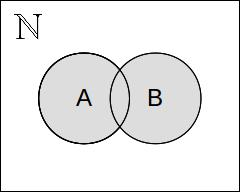
\includegraphics[scale=0.5]{Venn}
\caption{\label{fig:Venn-diagram}Representation of $A \cup B$ as a Venn Diagram}
\end{figure}

Given the sets $A$ and $B$, $A \backslash B$ is the \emph{set difference}\index{Set difference}, and ${A}^c$ is the \emph{complement}\index{Complement of a set} set of $A$. The \emph{De Morgan's laws} state that for every two sets $A$ and $B$ we have that $\left( A \cup B \right)^c = A^c \cap B^c$ and $\left( A \cap B \right)^c = A^c \cup B^c$.

Two sets $A$ and $B$ are \emph{disjoint}\index{Disjoint sets} if $A \cap B = \varnothing$. The sets $A_1, A_2, \ldots, A_n$ are disjoint if for every $i$ and $j$ such that $i \neq j$ we have that $A_i \cap A_j = \varnothing$. A \emph{partition}\index{Partition of a set} of a set $A$ is a collection of nonempty disjoint subsets of $A_1, A_2, \dots, A_n$ of $A$ such that  $A = \cup_{i=1}^n A_i$. The \emph{power set}\index{Power set} $\mathcal{P}(A)$ is the set whose members are all possible subsets of A. If $d(A)=n$ then $d\left( \mathcal{P}(A) \right) = 2^n$.

\begin{example}
Given the set $A = \{1, 2, 3\}$, its power set is:
\[
\mathcal{P}(A) = \{\varnothing, \{1\}, \{2\}, \{3\}, \{1,2\}, \{1,3\}, \{2,3\}, A\}
\]
\end{example}

Let $A$ be a non-empty set and $\mathcal{F}$ a collection fo subsets of $A$, the pair $\left( A, \mathcal{F} \right)$ is called an \emph{field}\index{Field of sets} over $A$ if the following properties are satisfied: it contains the empty set $\varnothing \in \mathcal{F}$, it is closed under complementation $F^c  \in \mathcal{F}$ for all $F \in \mathcal{F}$, and it is closed under finite unions $F_1 \cup \ldots \cup F_n  \in \mathcal{F}$ for all $F_1, \ldots, F_n \in \mathcal{F}$. It can be show that a field must satisfy the following two addtional properties: $A \in \mathcal{F}$ and $F_1 \cap \ldots \cap F_n  \in \mathcal{F}$ for all $F_1, \ldots, F_n \in \mathcal{F}$ (closed under finite intersections).

% Relations

Given $x$ and $y$, the \emph{ordered pair}\index{Ordered pair} $\left(x, y\right)$ consists of $x$ and $y$ in that order. An \emph{n-tuple}\index{n-tuple} is an $n$-ary ordered pair. The \emph{Cartesian product}\index{Cartesian product} of two sets $A$ and $B$, denoted by $A \times B$, is the set composed by all the ordered pairs $\left(x, y\right)$ such that $x \in A$ and $y \in B$. The extension of the Cartesian product to $n$ sets $A_1, A_2, \dots, A_n$ is represented by $A_1 \times A_2 \times \dots A_n$, and the \emph{n-fold Cartesian product} of $A$ with itself is denoted by $A^n$.

A subset $R \subseteq A \times A$ is called a \emph{binary relation}\index{Binary relation}; we use the notation $aRb$ to denote that $\left(a, b\right) \in R$. A binary relation is called \emph{reflexive}\index{Reflexive relation} if for all $a \in A$ we have that $aRa$. A binary relation is called \emph{symmetric}\index{Symmetric relation} if for all $a, b \in A$ we have that if $aRb$ then $bRa$. A binary relation in which $aRb$ and $bRa$ implies that $a = b$ is called \emph{antisymmetric}\index{Antisymmetric relation}. A binary relation is \emph{transitive}\index{Transitive relation} if for all $a, b, c \in A$ we have that if $aRb$ and $bRc$ then $aRc$. A binary relation is called \emph{total}\index{Total relation} if for all $a, b \in A$ either $aRb$ or $bRa$. Binary relations can be extended to two different sets $A$ and $B$ as a subset $R \subseteq A \times B$, and to \emph{n-ary} relations $R \subseteq A_1 \times A_2 \times \dots A_n$.

A binary relation $R \subseteq A \times A$ that is reflexive, symmetric and transitive is called an \emph{equivalence relation}. Equivalence relations are denoted by $\sim$. Two elements $a, b \in A$ are said to be \emph{equivalent} if they are related $a \sim b$. The \emph{equivalence class} of $a$, denoted by $[a]$, is composed by all the elements of $A$ that are equivalent to $a$, that is $[a] := \{ b \in A : a \sim b\}$. An equivalence relation partitions the underlying set into the \emph{quotient set} $A / {\mathord {\sim }} := \{ [a] : a \in A \}$.

A \emph{partial order} is a binary relation which is reflexive, transitive and antisymmetric; partial orders are represented by the symbol $\preceq$. A set with a partial order is called a \emph{partially ordered set} (also called a \emph{poset}).  An element $a \in A$ of a partially ordered set is \emph{minimal} if it does not exists another element $b \in A$ such that $b \preceq a$; an element $a \in A$ is \emph{maximal} if it does not exists another element $b \in A$ such that $a \preceq b$. A relation that is is reflexive, transitive, antisymmetric and total is called a \emph{total order}; total orders are represented by the symbol $\leq$. A set paired with a total order is called a \emph{totally ordered set}\index{Totally ordered set}. Given a totally ordered set $A$ we denote $\max(A)$ the \emph{maximum}\index{Maximum} element of $A$, and $\min(A)$ its \emph{minimum}\index{Minimum} element.

\begin{example}
Let $R \subset \mathbb{N} \times \mathbb{N}$ a relation such that $(a, b) \in R$ if $a$ divides $b$. $\mathbb{N}$ with $R$ is a partially ordered set. The number $11$ is a minimal element of $R$, since $11$ is a prime number.
\end{example}

% Functions

A \emph{function}\index{Function} is a binary relation $f \subseteq A \times B$ where for every $x \in A$ there is at most one $y \in B$ such that $\left(x, y\right) \in f$, the elements $\left(x, y\right) \in f$ are denoted by $f(x)=y$, and the function by $f : A \rightarrow B$. The set $A$ is called the \emph{domain}\index{Domain} of $f$, and $B$ the \emph{codomain}\index{Codomain}. The set $\{ y \in B : \exists x \in A , f(x) = y\}$ is the \emph{range}\index{Range} of $f$. A function is called \emph{partial}\index{Partial function} if the relation is not defined for all $x \in A$; we denoted by $f(x) \uparrow$ if the function $f$ is not defined for $x$. 

\begin{example}
In Section \ref{sec:computable_functions} we will see an alternative definition of the concept of function, as a procedure, or collection of steps, that asigns to the elements of $A$ an element of $B$. For example, the following C code defines a partial function from $\mathbb{R}$ to $\mathbb{R}$. It is partial because $inv(0)\uparrow$:
\begin{verbatim}
    double inv(double x) { return 1 / x }
\end{verbatim}
\end{example}

A function is \emph{injective}\index{Injective function} if for all $x$ and $y$ if $f(x) = f(y)$ then $x=y$. A function is \emph{surjective}\index{Surjective function} if for all $y$ there exists at least one $x$ such that $f(x) = y$. A function is \emph{bijective}\index{Bijective function} if it is both, injective and surjective. The \emph{identity}\index{Identity function} function $I_A : A \rightarrow A$, defined by $f(a) = a$ for all $a \in A$, is bijective. The concepts of function, partial function, injective, surjective and bijective can be easily generalized to $n$-ary relations.

Given a function $f$ the \emph{inverse}\index{Inverse function} function, denoted by $f^{-1}$, is defined by $f(f^{-1}(x)) = f^{-1}(f(x)) = x$. Given two functions $f$ and $g$, where the domain of $f$ is the range of $g$, we define the \emph{composition}\index{Composition} of $f$ with $g$, denoted by $f \circ g$, as $f \circ g = f(g(x))$.

An infinite set $A$ is \emph{countable}\index{Countable set} if there exists a bijective function between the elements of $A$ and the set of natural numbers $\mathbb{N}$. A set is \emph{uncountable}\index{Uncontable set} if it is neither finite nor countable. We say that a set has \emph{countable many}\index{Countable many set} elements if it is either finite or countable.

\begin{example}
$\mathbb{N}$, $\mathbb{Z}$ and $\mathbb{Q}$ are countable sets, $\mathbb{R}$ is not.
\end{example}

The \emph{characteristic function}\index{Characteristic function} of a set $A$ is the function $1_A : A \rightarrow \{1, 0\}$ defined as $1_A(x) = 1$ if $x \in A$ and $0$ otherwise.

Given a real number $x \in \mathbb{R}$, the \emph{absolute value}\index{Absolute value} of x, denoted $\mid x \mid$, is defined as $x$ is $x \geq 0$ and $-x$ if $x < 0$. The \emph{ceil}\index{Ceil} of $x$, denoted $\lceil x \rceil$ , is the least integer that is greater than or equal to $x$; the \emph{floor}\index{Floor} of $x$, denoted by $\lfloor x \rfloor$, is the greatest integer that is less than or equal to $x$. Given two positive integers $a$ and $b$, $a$ \emph{modulo} $b$, denoted by $a \bmod b$, is the remainder of the integer division of $a$ by $b$.

Let $f$ and $g$ be two functions $f,g:\mathbb{N}\rightarrow\mathbb{R}^{+}$. We say that $f(n)$ is of order of $g(n)$, denoted by $f(n)=O(g(n))$, if there exists positive integers $c$ and $m$ such that for every integer $n \geq m$ we have that $f(n)\leq cg(n)$. When $f(n)=O(g(n))$ we say that $g$ is an upper bound for $f$.

%
% Section: Strings
%

\section{Strings}
\label{sec:strings}

Let $\mathcal{S}=\left\{ s_{1},s_{2},\ldots,s_{q}\right\}$ be a non-empty finite set called \emph{alphabet}\index{Alphabet}. A \emph{sequence} over $\mathcal{S}$ is any ordered collection of symbols $x_1 x_2 \dots x_n$ from $\mathcal{S}$. When the alphabet is the set $\mathcal{B} = \{0, 1\}$, the sequences are called \emph{binary}. If the sequence is finite we call it \emph{string}\index{string}. In this book we will be working most of the time with binary strings. The \emph{length}\index{Length of a string} of a string $s$, denoted by $l(s)$, is the number of symbols in $s$. The \emph{empty string}\index{Empty string} is the unique string over $\mathcal{S}$ of length 0, and is denoted $\lambda$. Let $x \in \mathcal{S}$, by $x^n$ we denote the string $x x \ldots x$ ($n$-times). If $s = x_1 x_2 \dots x_n$ is a string, its \emph{reverse}\index{Reverse string} $s^R$ is $x_n x_{n-1} \dots x_1$.

Let $\mathcal{S}^{n}$ denote the set of all strings $s_{1}s_{2}\ldots s_{n}$ of length $n$\footnote{Do not confuse the set of strings of length $n$ over an alphabet $\mathcal{S}^n$ with the $n$-fold Cartesian product of a set $S^n$, alphabets will be represented by using calligraphic fonts.}, $\mathcal{S}^{+}=\cup_{n\geq1}\mathcal{S}^{n}$ and $\mathcal{S}^{\ast} = \mathcal{S}^{+} \cup \{\lambda\}$. Note that all the strings that belong to $\mathcal{S}^{\ast}$ have finite lengths. $\mathcal{S}^{\ast}$ is called the Kleene \emph{closure} of $\mathcal{S}$.

\begin{example}
The following relations hold: $d \left( \left\{ s \in \mathcal{B}^{\ast} : l(s) = n \right\} \right) = 2^n$ and $d \left( \left\{ s \in \mathcal{B}^{\ast} : l(s) \leq n \right\} \right) = 2^{n+1}-1$.
\end{example}

For any two strings $s$ and $t$ in $\mathcal{S}^{\ast}$, the \emph{concatenation}\index{String concatenation} of $s$ and $t$, denoted by $st$, is defined as the sequence of symbols in $s$ followed by the sequence of symbols in $t$. Note note that $l(st) = l(s) + l(t)$. $S^\ast$ is closed under the operation of concatenation. $S^\ast$ with the operation of concatenation forms a \emph{free monoid}, that it, it is associative  $s(tr)=(st)r$, and has an identity element $\lambda a = a \lambda = a$.

A string $s$ is said to be a \emph{substring}\index{Substring} of $t$ if there exist (possibly empty) strings $u$ and $v$ such that $t$ = $usv$. A string $s$ is said to be a \emph{prefix}\index{Prefix} of $t$, denoted by $s <_p t$, if there exists a string $u$ such that $t = su$. A subset $S \subset \mathcal{S}^{\ast}$ is \emph{prefix free}\index{Prefix free set} if for all $s, t \in S$, if $s <_p t$ then $s = t$. Given a string $s \in \mathcal{S}^{\ast}$, the \emph{self delimited}\index{Self delimited string} version of $s$, denoted by $\bar{s}$, is $\bar{s} = 1^{l(s)}0s$. Note that $l(\bar{s}) = 2l(s)+1$.

\begin{example}
The set $\bar{\mathcal{S}^{\ast}}$composed by all the self delimited strings of $\mathcal{S}^{\ast}$ is prefix free.
\end{example}

If $\mathcal{S}$ is a total ordered set, we can define a total order on $\mathcal{S}^{\ast}$, called \emph{shortlex ordering}\index{Shortlex ordering}, in which sequences are primarily sorted by length with the shortest sequences first, and sequences of the same length are sorted into their lexicographical order.

\begin{example}
If $S = \{a, b, c\}$ and $a < b < c$, then the shortlex order on $\mathcal{S}^{\ast}$ includes the relations $\lambda < a < b < c < aa < ab < \ldots < cc < aaa < aab < \ldots < ccc < \ldots$
\end{example}

Given an arbitrary object $O$ we denote its representation as a string as $\left\langle O\right\rangle$, assuming that there exists an standard encoding method. Given the objects $O_{1},O_{2},\ldots,O_{k}$, the concatenation of the representations of these objects $\left\langle O_1 \right\rangle \left\langle O_2 \right\rangle \ldots \left\langle O_k \right\rangle$ is denoted by $\left\langle O_1 O_2 \ldots O_k \right\rangle$. The concatenation of the representation of these objects in such a way that we can decode and uniquely identify all of them is represented by $\left\langle O_1, O_2,\ldots,O_k \right\rangle$, for example, we could use $\left\langle O_1, O_2,\ldots,O_k \right\rangle = \bar{\left\langle O_1 \right\rangle} \bar{\left\langle O_2 \right\rangle} \ldots \bar{\left\langle O_k \right\rangle}$.

\begin{example}
Natural numbers can be represented by binary strings using the following encoding method: $\langle 0 \rangle = \lambda$, $\langle 1 \rangle \rightarrow 0$, $\langle 2 \rangle \rightarrow 1$, $\langle 3 \rangle \rightarrow 00$, $\langle 4 \rangle \rightarrow 01$, $\langle 5 \rangle \rightarrow 10$, $\langle 6 \rangle \rightarrow 11$, $7 \rightarrow 000$, ... For example $\left\langle 3, 7 \right\rangle$  would be represented as $110001110000$. Given this encoding we have that $l \left( \langle n \rangle \right) = \lfloor \log_2 (n + 1) \rfloor$.
\end{example}

%
% Section: Matrices
%

\section{Matrices}
\label{sec:preliminaries-matrices}

A \emph{matrix} $A$ of order $m \times n$ is a set of $mn$ scalars ordered in $m$ \emph{rows} and $n$ \emph{colums} in the following way:
\[
A = 
 \begin{pmatrix}
  a_{1,1} & a_{1,2} & \cdots & a_{1,n} \\
  a_{2,1} & a_{2,2} & \cdots & a_{2,n} \\
  \vdots  & \vdots  & \ddots & \vdots  \\
  a_{m,1} & a_{m,2} & \cdots & a_{m,n} 
 \end{pmatrix}
\]
The \emph{entry} $a_{ij}$ corresponds to the element of $A$ localed at row $i$ and column $j$. We denote by $\mathcal{M}_{m \times n}$ the \emph{set of all matrices} of order $m \times n$. A \emph{row matrix} is a matrix that belongs to $\mathcal{M}_{1 \times n}$, and a \emph{column matrix} to $\mathcal{M}_{m \times 1}$. A \emph{squared matrix} is a matrix that belongs to $\mathcal{M}_{n \times n}$. The entries $a_{ii}$ form the \emph{main diagonal} of a square matrix. The \emph{transpose matrix} of a matrix $A \in \mathcal{M}_{m \times n}$ is the matrix $A^T \in \mathcal{M}_{n \times m}$ whose entries $(i,j)$ are equal to the entries $(j, i)$ of $A$. If $A = A^T$ we say that $A$ is a \emph{symmetric matrix}. A \emph{diagonal matrix} is a matrix whose all its entries outside the main diagonal are zero. The \emph{identity matrix} $I$ is a diagonal squared matrix with all the entries in the main diagonal equal to 1. A \emph{submatrix} of a matrix is obtained by deleting any collection of rows and/or columns.

\begin{example}
Given the squared matrix $A = \left( \begin{smallmatrix} 1 & 2 & 3 \\ 4 & 5 & 6 \\ 7 & 8 & 9 \end{smallmatrix} \right)$ we have that the entry $(2, 3)$ has the value $6$, the diagonal is composed by the numbers $1$, $5$, and $9$, its transpose is $A^T = \left( \begin{smallmatrix} 1 & 4 & 7 \\ 2 & 5 & 8 \\ 3 & 6 & 9 \end{smallmatrix} \right)$, and that the matrix $B = \left( \begin{smallmatrix} 1 & 3 \\ 4 & 6 \end{smallmatrix} \right)$ is a submatrix of $A$.
\end{example}

The sum of two matrices $A$ and $B$ of equal size is the matrix $A + B$ whose entry $(i, j)$ are $(A + B)_{ij} = a_{ij} + b_{ij}$. The operation of sum of matrices is associative $(A + B) + C = A + (B + C)$, commutative $A + B = B + A$, has a neutral element $A + 0_{m \times n} = A$ and an inverse element $A + (-A) = 0_{m \times n}$. The multiplication of a scalar $\lambda$ by a matrix $A$ is the matrix $\lambda A$ whose entry $(i, j)$ is $(\lambda A)_{ij} = \lambda a_{ij}$. The operation of multiplication of a scalar by a matrix is distributive with respect to the sum of matrices $\alpha (A + B) = \alpha A + \alpha B$, distributive with respect to the sum of scalars $(\alpha + \beta) A = \alpha A + \beta B$, associative with respect to the product by scalars $(\alpha \beta) A = \alpha (\beta A)$, and has a unit element $1 A = A$. The product of two matrices $A_{m \times n}$ and $B_{n \times p}$ is the matrix $AB_{m \times p}$ whose entry $(i, j)$ is $(AB)_{ij} = \sum_{k=1}^n a_{ik} b_{kj}$. The operation of multiplication of matrices is associative $(A B) D = A (B D)$, has a left neutral element $A I_n = A$ and a right neutral element $I_m A = A$, associative with respect to the product by scalars $\alpha (A B) = (\alpha A) B = A (\alpha B)$, distributive with respect the sum of matrices by the right $A (B + C) = AB + AC$ and the left $(B + C) D = B D + C D$. Additionally, the operation of traspose satisfies the following properties: $(A + B)^T = A^T + B^T$, $(\lambda A)^T = \lambda A^T$, $(A B)^T = B^T A^T$.

\begin{example}
Given the matrices $A = \left( \begin{smallmatrix} 1 & 2 \\ 3 & 5 \end{smallmatrix} \right)$ and $B = \left( \begin{smallmatrix} 5 & 6 \\ 7 & 8 \end{smallmatrix} \right)$ we have that $A + B = \left( \begin{smallmatrix} 6 & 8 \\ 10 & 13 \end{smallmatrix} \right)$, $2 A = \left( \begin{smallmatrix} 2 & 4 \\ 6 & 10 \end{smallmatrix} \right)$ and $A B = \left( \begin{smallmatrix} 19 & 22 \\ 50 & 58 \end{smallmatrix} \right)$.
\end{example}


%
% Section: Graphs
%

\section{Graphs}
\label{sec:Graphs}

A \emph{graph}\index{Graph}\footnote{The definition of graph provided in this introduction is equivalent to the definition of \emph{simple graph} in the standard discrete mathematics literature.} $G$ is an ordered pair $(V,E)$ composed by a nonempty set of objects $V$, called \emph{vertices}\index{Vertices of a graph}, connected by set of links $E$, called \emph{edges}\index{Edges of a graph}. The elements of $E$ have the form of unordered pairs $\left\{ u,v\right\}$ of distinct (no loops allowed) vertices $u$,$v\in V$. Vertices $u$ and $v$ are said to be \emph{adjacent}\index{Adjacent vertices} if there is and edge $\left\{ u,v\right\} \in E$, and if so, they are called the \emph{endpoints}\index{Endpoints of an edge} of the edge. If the set $V$ is infinite, the graph is called \emph{infinite graph}\index{Infinite graph}; however, in this book we will consider only finite graphs. If the pairs of vertices $u, v$ are ordered pairs, the graph is called \emph{directed graph}\index{Directed graph}, and in that case, $u$ is called the \emph{initial vertex}\index{Initial vertex} and $v$ the \emph{terminal vertex}\index{Terminal vertex}. If $G = (V,E)$ is a graph, its \emph{adjacency matrix}\index{Adjacency matrix} is a square $d(V) \times d(V)$ matrix $A$ such that the element $A_{uv}$ is 1 if $\left\{ u,v\right\} \in E$ and 0 otherwise.

Graphs are usually depicted as a set of dots for the vertices, joined by lines for the edges. If the graph is directed, we use arrows instead of lines to represent edges.

\begin{example}
Let $V=\{a, b, c, d\}$ and $E=\{ \{a,b\}, \{a,c\}, \{a,d\}, \{b,c\} \}$, the graph $G=(V,E)$ is depicted in Figure \ref{fig:Graph-Example}.
\end{example}

\begin{figure}[h]
\centering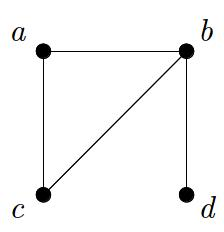
\includegraphics[scale=0.5]{GraphExample}
\caption{\label{fig:Graph-Example}An Example of Graph}
\end{figure}

If $v$ is an endpoint of and edge $e$, then we say that $e$ is is \emph{incident}\index{Incident edge} on $v$. The \emph{degree}\index{Degree of a vertex} of a vertex $v$, written $\deg(v)$, is equal to the number of edges which are incident on $v$. A vertex of degree zero is called \emph{isolated}\index{Isolated vertex}; a vertex of degree one is called \emph{pendant}\index{Pendant vertex}. The \emph{neighborhood}\index{Neighborhood of a vertex} of vertex $v$, denoted by $N(v)$, is the set of all vertices that are adjacent to $v$. If $A \subset V$, the neighborhood of $A$ is $N(A) = \cup_{v \in A} N(v)$. If $G$ is directed graph, we call the \emph{in-degree}\index{In-degree of a vertex} of a vertex $v$, denoted by $indeg(v)$, to the number of edges in which $v$ is an terminal vertex, and \emph{out-degree}\index{Out-degree of a vertex}, denoted by $outdeg(v)$, to the number of edges in which $v$ is an initial vertex. A \emph{path}\index{Path} in a graph is a sequence of distinct vertices $\{v_{0}, v_{1}, \ldots ,v_{k}\}$ in which $v_{i}$ and $v_{i+1}$ are adjacent for each $1 \leq i < k$. If $v_{0} = v_{k}$ we say that the path is a \emph{cycle}\index{Cycle}.

\begin{example}
Given a graph $G=(V,E)$, the \emph{handshaking theorem}\index{Handshaking theorem} states that $\sum_{v \in V} deg(v) = 2 m$, where $m = d(E)$, since each edge has two end points.
\end{example}

A graph $G$ is said to be \emph{bipartite}\index{Bipartite graph} if the set of vertices $V$ can be partitioned into two subsets $V_1$ and $V_2$ such that each edge of $G$ connects a vertex of $V_1$ to a vertex of $V_2$. Bipartite graphs are usually denoted by $G=(V_1, V_2, E)$. The degree of the vertices of a bipartite graph satisfied the following property, called the \emph{degree sum formula}\index{Degree sum formula}, $\sum_{u \in V_1} deg(u) = \sum_{v \in V_2} deg(v) = d(E)$.

A graph $G(V',E')$ is a \emph{subgraph}\index{Subgraph} of $G(V,E)$ if $V'$ is a subset of $V$ and $E'$ is a subset of $E$ whose endpoints belong to $V'$. A graph $G$ is called a \emph{labeled graph}\index{Labeled graph} if its edges and/or vertices are assigned data of one kind or another. In particular, if each edge $e$ of $G$ is assigned a nonnegative number $w(e)$ then $w(e)$ is called the \emph{weight}\index{Weight of an edge} of $e$.

A particular type of graph that will be extensively used in this book are trees. A \emph{tree}\index{Tree} is a non-empty graph in which any two vertices are connected by a unique path. Given a tree, we will always designate a particular vertex, called the \emph{root}\index{Root of a tree} of the tree, and direct each edge away from that root.

\begin{example}
An equivalent definition of trees is provided by set theory. According to set theory a tree is a partially ordered set $(T, <)$ such that for each $t \in T$, the set $S = \{ s \in T : s < t \}$ has an element that is smaller than every other element of S (\emph{least element}).
\end{example}

Let $T$ be a tree. If $v$ is a vertex in $T$ other than the root, the \emph{parent}\index{Parent of a vertex} of $v$ is the unique vertex $u$ such that there is an edge connecting $u$ to $v$. If $u$ is the parent of $v$, then $v$ is called a \emph{child}\index{Child of a vertex} of $u$. A \emph{sibling}\index{Sibling to a vertex} to a vertex $v$ is any other vertex on the tree which has the same parent than $v$. The \emph{ancestors}\index{Ancestors of a vertex} of a vertex are the vertices in the path from the root to this vertex, excluding the vertex itself and including the root. The \emph{descendants}\index{Descendant of a vertex} of a vertex $v$ are those vertices that have $v$ as an ancestor. A vertex is called a \emph{leaf}\index{Leaf vertex} if it has no children. Vertices that have children are called \emph{branches}\index{Branches of a tree}. The \emph{depth}\index{Depth of a vertex} of a vertex $v$ is the length of the unique path from the root to $v$. The \emph{height}\index{Height of a tree} of a tree is the maximum of the levels of its vertices. 

\begin{example}
The following applies to the tree depicted in Figure \ref{fig:BinaryTree-Example}: the root is the vertex $a$; $c$ is a parent of $d$ and $d$ is a child of $c$; $d$ and $g$ are siblings; the ancestors of $d$ are $a$ and $c$; the descendants of $c$ are $e$, $e$ and $f$; $b$, $e$, $f$ and $g$ are leaf nodes; $c$ and $d$ are branches; the depth of $d$ is 3; the height of the tree is 4.
\end{example}

\begin{figure}[h]
\centering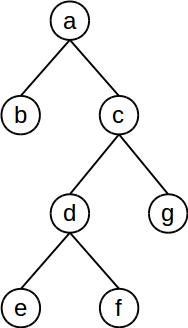
\includegraphics[scale=0.5]{BinaryTree}
\caption{\label{fig:BinaryTree-Example}An Example of Tree}
\end{figure}

If $v$ is a vertex in a tree, the \emph{subtree}\index{Subtree} with $v$ as root is the subgraph of the tree consisting of $v$ and its descendants and all edges incident to these descendants. A tree is called an \emph{k-ary tree}\index{k-ary tree} if every branch has not more than $k$ children. The tree is called a \emph{full k-ary tree}\index{full k-ary tree} if every branch has exactly $k$ children. An \emph{k-ary} tree with $k=2$ is called a \emph{binary tree}\index{Binary tree}. A $k$-ary tree of height $h$ is \emph{balanced}\index{Balanced tree} if all its leaves are have a depth of $h$ or $h-1$.

\begin{example}
A tree with $n$ vertices has $n-1$ edges. A full $k$-ary tree with $i$ branches contains $m=ki+1$ vertices.
\end{example}

{\color{red} TODO: Mention tree-traversals algorithms.}

%
% Section: Counting Methods
%

\section{Counting Methods}
\label{sec:counting}








\section*{References}

Two easy to read books on discrete mathematics that cover what it is covered in this chapter and part of the the following chapters are \cite{rosen1995discrete} and \cite{epp2010discrete}. Good introductions to statistics and the theory of probability are \cite{degroot1986probability} and \cite{spiegel2012probability}.
